% Chapter 1

\chapter{Clustering} % Main chapter title

\label{Chapter8} % For referencing the chapter elsewhere, use \ref{Chapter1} 

\lhead{Chapter 8. \emph{Clustering}} % This is for the header on each page - perhaps a shortened title

%----------------------------------------------------------------------------------------

\section{Importance of feature selection }

 Feature selection in the context of clustering refers to the process of choosing a subset of relevant features from the original set of features in a dataset before applying a clustering algorithm. This selection is performed to enhance the quality of clustering results and improve the efficiency of the clustering process.
 
 \section{Selection of features and reasoning}
 I selected: 'Unit price', 'Quantity', 'Tax 5\%', 'Total', 'cogs', 'gross income' and 'Rating'. 
 \newline 
Features like 'Unit price', 'Quantity', and 'Total', are likely to capture essential aspects of customer transactions. 'Rating' could provide insights into customer satisfaction. In addition to this, all the features I chose are commonly associated with sales transactions and customer behavior in retail. An alternative could’ve been employing some feature selection technique, like PCA. However, for this specific task, I chose to deal manually with feature selection.
\newline 
For all the plots, I’ve used the features ‘Total’ and ‘Rating’ for the axes.


\section{Why a standardized dataset is required:}
Standardization deals with issues related to scale disparities among features, which can significantly impact the performance of distance-based algorithms like KMeans. By transforming data to a common scale, standardization prevents biases toward features with larger magnitudes, enhances convergence, and facilitates meaningful comparisons. It also promotes model interpretability by ensuring that cluster centroids represent average values across features consistently. 

\section{Applying Clustering}
\subsection{Kmeans}
K-Means is a popular partitioning algorithm that divides a dataset into K clusters. It aims to minimize the sum of squared distances between data points and the centroid of their assigned cluster. It assigns each data point to the cluster with the nearest centroid.


\begin{table}[htbp]
    \centering
    \begin{adjustbox}{max width=\textwidth}
    \rowcolors{1}{green!20}{white}
    \begin{tabular}{|>{\columncolor{green!50}}c|c|}
        \hline
        \rowcolor{green!70}
        \textbf{Metric Name} & \textbf{Score} \\
        \hline
        Inertia (K-Means) & 2705.273033683108 \\
        Silhouette Score & 0.3037813725498845 \\
        Davies-Bouldin Index  & 1.1812055382786706 \\
        Calinski-Harabasz Index  & 791.3882872643744 \\
        \hline
    \end{tabular}
    \end{adjustbox}
    % \caption{5 by 2 Table with Light Green Alternating Row Colors}
    \label{tab:green_table}
\end{table}

The numbers indicate a moderate level of compactness (Inertia: 2705.27) and well-defined clusters, as indicated by the Silhouette Score (0.30), Davies-Bouldin Index (1.18), and Calinski-Harabasz Index (791.39). These metrics collectively suggest that the chosen number of clusters (3) is appropriate for grouping customers based on their purchase history. The clusters exhibit reasonable separation and distinctiveness, providing valuable insights for customer segmentation.

\begin{figure}[h]
    \centering
    \begin{minipage}{0.45\textwidth}
        \centering
        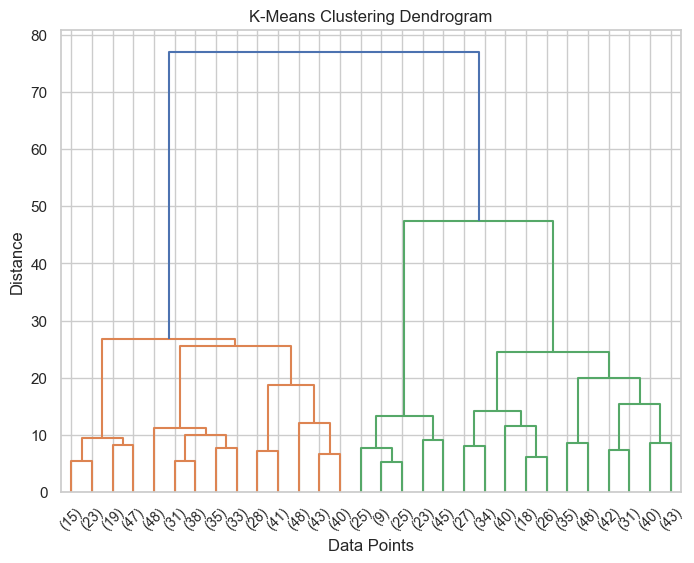
\includegraphics[width=\linewidth]{Chapters/ch8/ch_8_kmeans_dendo.png}
        \caption{Dendrogram}
        \label{fig:dendrogram}
    \end{minipage}\hfill
    \begin{minipage}{0.45\textwidth}
        \centering
        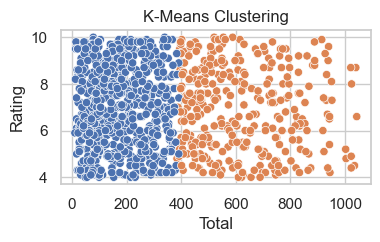
\includegraphics[width=\linewidth]{Chapters/ch8/ch_8_kmeans_scatter.png}
        \caption{Scatterplot}
        \label{fig:scatterplot}
    \end{minipage}
\end{figure}



% ----------------------------------------------------------------------------------------


\subsection{K-Median}
Like K-Means, K-Median is a partitioning algorithm that seeks to minimize the sum of absolute differences (medians) between data points and the centroid of their assigned cluster. K-Median is more robust to outliers compared to K-Means.

\begin{figure}[h]
    \centering
    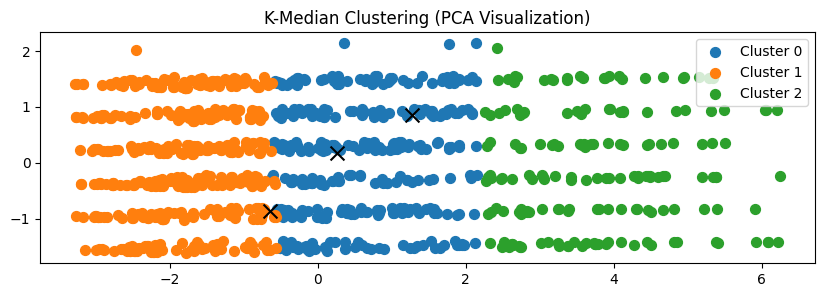
\includegraphics[width=0.7\textwidth]{Chapters/ch8/ch_8_kmedian_scatter (2).png}
    \caption{Scatter plot}
    % \label{fig:example}
\end{figure}

\subsection{ARI and NMI}
\begin{table}[htbp]
    \centering
    \begin{adjustbox}{max width=\textwidth} % Fit the table to the page width
        \rowcolors{1}{green!20}{white} % Alternate row colors starting from the second row
        \rowcolors{2}{green!30}{white} % Slightly darker header row
        \begin{tabular}{|>{\columncolor{green!50}}c|c|}
            \hline
            \rowcolor{green!50} % Slightly darker header row color
            \textbf{Metric} & \textbf{Score} \\
            \hline
            Adjusted Rand Index (ARI) & 0.5451 \\
            Normalized Mutual Information (NMI) & 0.5859 \\
            \hline
        \end{tabular}
    \end{adjustbox}
    % \caption{3 x 2 Table with alternating light green rows and a slightly darker green header}
    \label{tab:3x2_table}
\end{table}
The Adjusted Rand Index (ARI) measures the similarity between clusters obtained by different algorithms. A score of 0.5451 indicates a moderate agreement between K-Means and Agglomerative Clustering.
\newline
Normalized Mutual Information (NMI) measures the mutual dependence between clusters. The score of 0.5859 suggests a reasonable degree of similarity between the two clustering methods.

% \newpage
% \subsection{results}
The similarity in results between K-Means and Agglomerative Clustering suggests that both algorithms capture similar patterns in the data. 
\begin{figure}[h]
    \centering
    \begin{minipage}{0.45\textwidth}
        \centering
        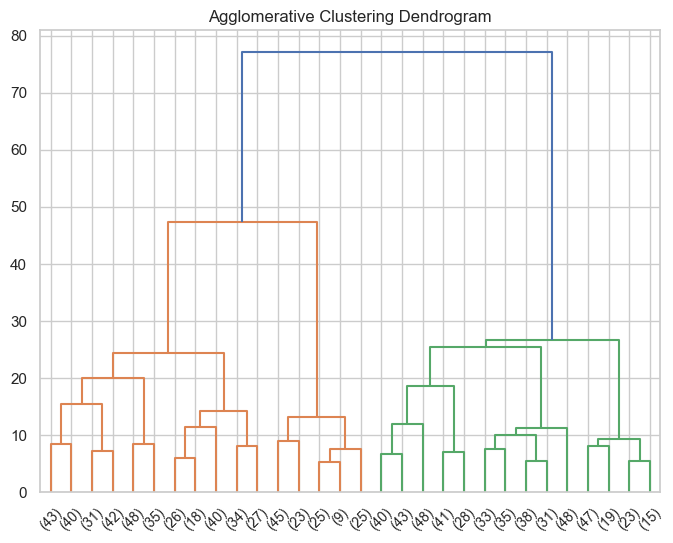
\includegraphics[width=\linewidth]{Chapters/ch8/ch_8_agglo_dendo.png}
        \caption{Dendrogram}
        \label{fig:dendrogram}
    \end{minipage}\hfill
    \begin{minipage}{0.45\textwidth}
        \centering
        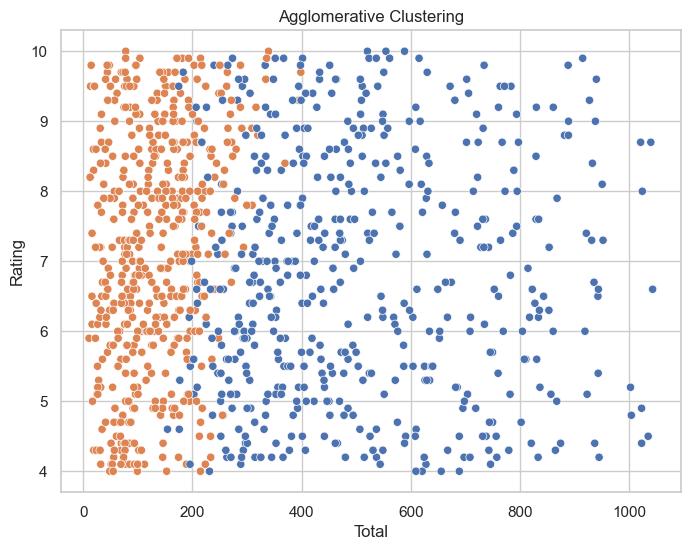
\includegraphics[width=\linewidth]{Chapters/ch8/ch_8_agglo_scatter.png}
        \caption{Scatterplot}
        \label{fig:scatterplot}
    \end{minipage}
\end{figure}



% -------------------------------------------------------------------------------------------------------------
\subsection{DBSCAN:}

\begin{table}[htbp]
    \centering
    \begin{adjustbox}{max width=\textwidth} % Fit the table to the page width
        \rowcolors{1}{green!20}{white} % Alternate row colors starting from the second row
        \rowcolors{2}{green!30}{white} % Slightly darker header row
        \begin{tabular}{|>{\columncolor{green!50}}c|c|}
            \hline
            \rowcolor{green!50} % Slightly darker header row color
            \textbf{Metric} & \textbf{Score} \\
            \hline
            Silhouette Score (DBSCAN)  & 0.12528450383737091 \\
            Davies-Bouldin Index (DBSCAN)  & 1.5543217530912334 \\
            Number of Clusters (DBSCAN) & 23 \\
            \hline
        \end{tabular}
    \end{adjustbox}
    % \caption{3 x 2 Table with alternating light green rows and a slightly darker green header}
    \label{tab:3x2_table}
\end{table}

In applying DBSCAN to cluster customers based on purchase history, the algorithm identified 23 clusters. However, the negative Silhouette Score of approximately -0.125 indicates potential overlap between clusters, while the Davies-Bouldin Index of around 1.55 suggests moderate separation. These results may be indicative of the algorithm's sensitivity to data density and its tendency to partition the dataset into numerous, potentially small, dense regions. 

\begin{figure}[h]
    \centering
    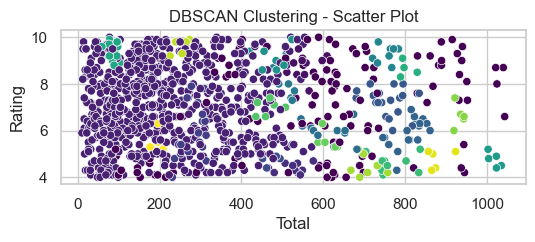
\includegraphics[width=0.7\textwidth]{Chapters/ch8/ch_8_dbscan_scatter.png}
    \caption{scatter plot}
    % \label{fig:examle}
\end{figure}

% \section{Mean Shift}
% \begin{figure}[h]
%     \centering
%     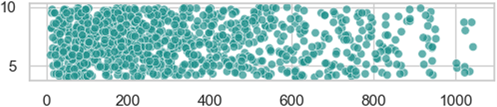
\includegraphics[width=0.7\textwidth]{Chapters/ch8/scatterplot_5.png}
%     % \caption{Radar graph}
%     % \label{fig:example}
% \end{figure}
% The single-cluster prediction by Mean Shift indicates its unsuitability for the task at hand. Mean Shift's sensitivity to overall data density and homogeneity may lead to oversimplification and a failure to discern distinct clusters in the presence of irregularly shaped or non-convex structures.



% ------------------------------------------------------------------------------------------
